\documentclass[border=5pt]{standalone}
\usepackage{tikz}
\usepackage{pgfplots}
\pgfplotsset{compat=1.18}
\usepackage{xcolor}
\usepackage{amsmath}
\usepackage{amssymb}

% === BRAND COLORS ===
\definecolor{tiger}{HTML}{FF5A00}
\definecolor{fire}{HTML}{FF4D00}
\definecolor{flicker}{HTML}{DC4B07}
\definecolor{steel}{HTML}{878F92}
\definecolor{gunmetal}{HTML}{122128}
\definecolor{panel}{HTML}{202E35}

% === FIGURE COLORS ===
\definecolor{darknavy}{HTML}{122128}
\definecolor{forgisorange}{HTML}{FF5A00}
\definecolor{forgisfire}{HTML}{FF4D00}
\definecolor{forgisflicker}{HTML}{DC4B07}
\definecolor{figblue}{HTML}{3A7BD5}
\definecolor{figgreen}{HTML}{2ECC71}
\definecolor{figsteel}{HTML}{878F92}
\definecolor{panelbg}{HTML}{F0F4F8}
\definecolor{warmamber}{HTML}{FFF3CD}
\definecolor{figwhite}{HTML}{FFFFFF}

% === LEVEL COLORS ===
\definecolor{L1bg}{HTML}{E0F2F1}
\definecolor{L1border}{HTML}{00796B}
\definecolor{L2bg}{HTML}{FFF8E1}
\definecolor{L2border}{HTML}{F57F17}
\definecolor{L3bg}{HTML}{F3E5F5}
\definecolor{L3border}{HTML}{6A1B9A}
\definecolor{L4bg}{HTML}{FFEBEE}
\definecolor{L4border}{HTML}{B71C1C}

% === STEP TINT COLORS ===
\definecolor{step1bg}{HTML}{EBF2FA}
\definecolor{step1border}{HTML}{3A7BD5}
\definecolor{step2bg}{HTML}{E8F8EE}
\definecolor{step2border}{HTML}{2ECC71}
\definecolor{step3bg}{HTML}{FFF0E6}
\definecolor{step3border}{HTML}{FF5A00}

\definecolor{mutedgray}{HTML}{878F92}
\definecolor{chipborder}{HTML}{C0C8CE}

\usetikzlibrary{arrows.meta, calc, positioning, shapes.misc, fit, decorations.pathreplacing, backgrounds}

\tikzset{
    roundbox/.style 2 args={rounded corners=6pt, draw=#1, line width=0.8pt, fill=#2, inner sep=8pt},
    stepbox/.style 2 args={rounded corners=6pt, draw=#1, line width=1pt, fill=#2, inner sep=0pt, minimum width=4.8cm},
    chip/.style={rounded corners=2pt, draw=chipborder, fill=white, inner sep=2pt, font=\sffamily\fontsize{6}{7}\selectfont\ttfamily, minimum height=14pt},
    pill/.style={rounded corners=3pt, inner sep=2.5pt, font=\sffamily\fontsize{6}{7}\selectfont\bfseries, minimum height=14pt},
    subcard/.style={rounded corners=3pt, draw=chipborder, fill=white, inner sep=5pt, line width=0.5pt},
    mainarrow/.style={-{Stealth[length=5pt,width=4pt]}, line width=1.2pt, darknavy},
    successarrow/.style={-{Stealth[length=4pt,width=3pt]}, line width=0.8pt},
    numbercircle/.style={circle, fill=#1, text=white, font=\sffamily\bfseries\fontsize{7}{8}\selectfont, inner sep=0pt, minimum size=16pt},
}

\begin{document}
\sffamily
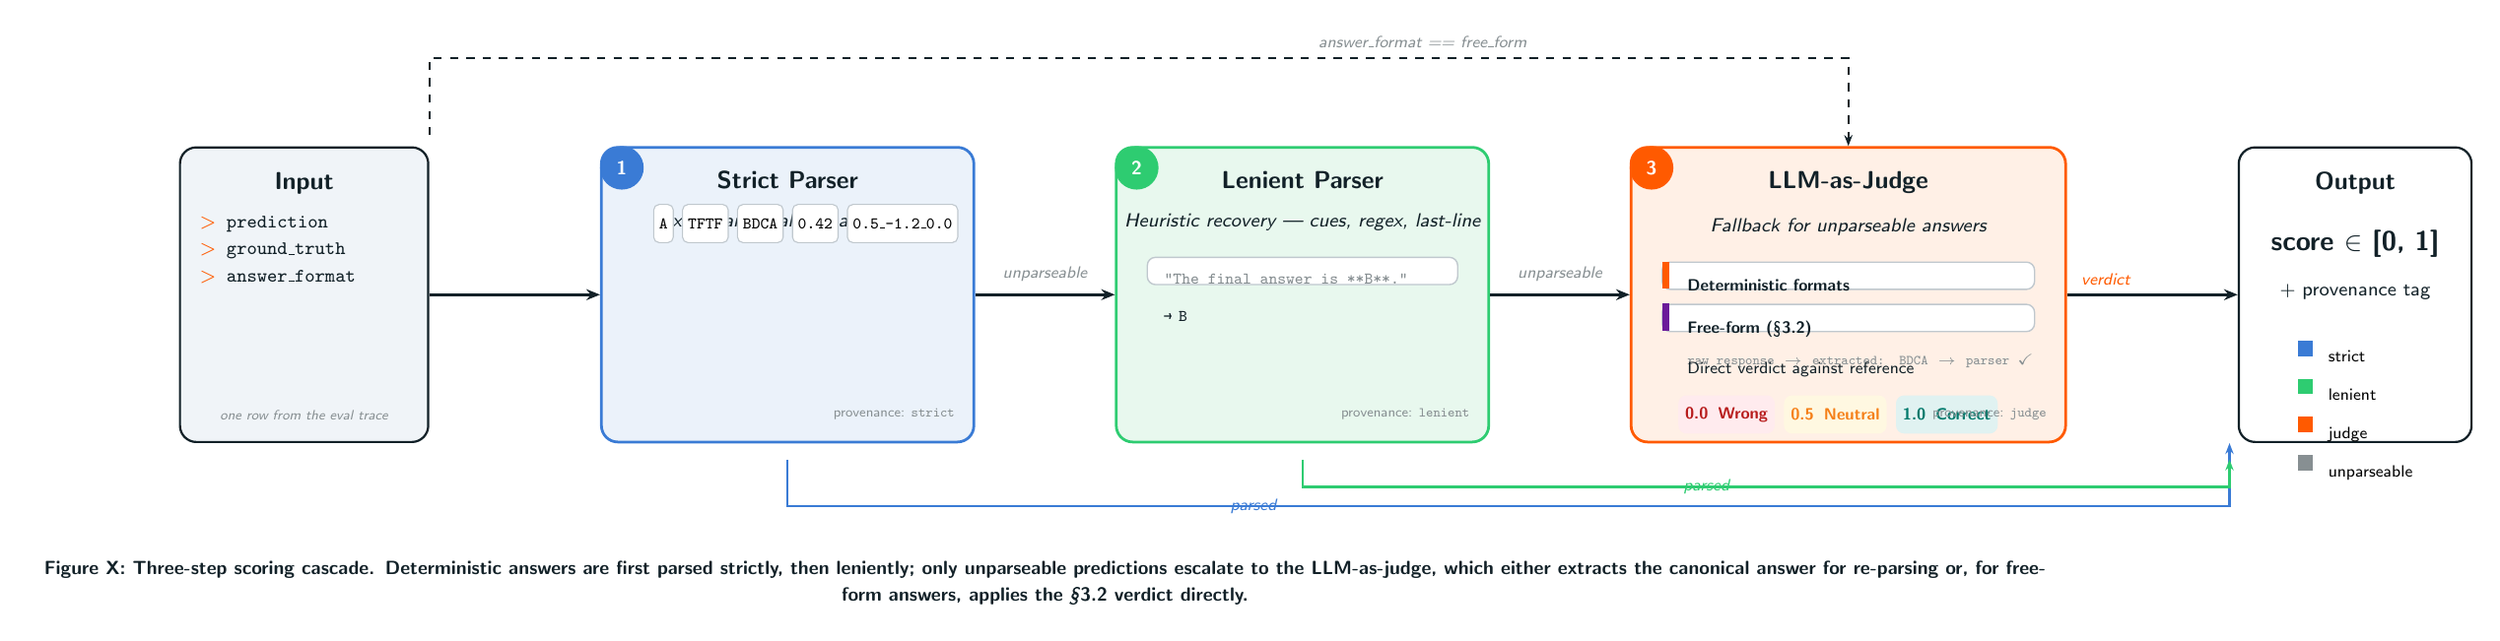
\begin{tikzpicture}[
    every node/.style={font=\sffamily},
]

% ============================================================
% ZONE 0: INPUT
% ============================================================
\node[roundbox={darknavy}{panelbg}, minimum width=3.2cm, minimum height=3.8cm, anchor=west] (input) at (0,0) {};
\node[font=\sffamily\bfseries\fontsize{9}{10}\selectfont, text=darknavy, anchor=north] at ([yshift=-6pt]input.north) {Input};
\node[font=\ttfamily\fontsize{7}{9}\selectfont, text=darknavy, anchor=north west, align=left] (inputlines) at ([shift={(4pt,-22pt)}]input.north west) {%
\textcolor{forgisorange}{\textgreater}~prediction\\[1pt]%
\textcolor{forgisorange}{\textgreater}~ground\_truth\\[1pt]%
\textcolor{forgisorange}{\textgreater}~answer\_format};
\node[font=\sffamily\itshape\fontsize{5.5}{6.5}\selectfont, text=mutedgray, anchor=south] at ([yshift=5pt]input.south) {one row from the eval trace};

% ============================================================
% ZONE 1: STRICT PARSER
% ============================================================
\node[stepbox={step1border}{step1bg}, minimum height=3.8cm, minimum width=4.8cm, anchor=west] (step1) at ([xshift=2.2cm]input.east) {};
\node[numbercircle=step1border] at ([shift={(8pt,-8pt)}]step1.north west) {1};
\node[font=\sffamily\bfseries\fontsize{9}{10}\selectfont, text=darknavy, anchor=north] (s1title) at ([yshift=-6pt]step1.north) {Strict Parser};
\node[font=\sffamily\itshape\fontsize{7}{8}\selectfont, text=darknavy, anchor=north] (s1sub) at ([yshift=-2pt]s1title.south) {Exact canonical-format match};

% Format chips
\node[chip] (chipA) at ([shift={(-1.6cm,-1.0cm)}]step1.north) {A};
\node[chip, right=3pt of chipA] (chipTF) {TFTF};
\node[chip, right=3pt of chipTF] (chipBD) {BDCA};
\node[chip, right=3pt of chipBD] (chip042) {0.42};
\node[chip, right=3pt of chip042] (chipVec) {0.5\_-1.2\_0.0};

\node[font=\sffamily\fontsize{5.5}{6.5}\selectfont, text=mutedgray, anchor=south east] at ([shift={(-4pt,5pt)}]step1.south east) {provenance: \texttt{strict}};

% ============================================================
% ZONE 2: LENIENT PARSER
% ============================================================
\node[stepbox={step2border}{step2bg}, minimum height=3.8cm, minimum width=4.8cm, anchor=west] (step2) at ([xshift=1.8cm]step1.east) {};
\node[numbercircle=step2border] at ([shift={(8pt,-8pt)}]step2.north west) {2};
\node[font=\sffamily\bfseries\fontsize{9}{10}\selectfont, text=darknavy, anchor=north] (s2title) at ([yshift=-6pt]step2.north) {Lenient Parser};
\node[font=\sffamily\itshape\fontsize{7}{8}\selectfont, text=darknavy, anchor=north] (s2sub) at ([yshift=-2pt]s2title.south) {Heuristic recovery --- cues, regex, last-line};

% Example card
\node[subcard, minimum width=4.0cm, anchor=north] (excard) at ([yshift=-6pt]s2sub.south) {};
\node[font=\ttfamily\fontsize{6.5}{8}\selectfont, text=mutedgray, anchor=north west, align=left] (exline1) at ([shift={(3pt,-3pt)}]excard.north west) {%
"The final answer is **B**."};
\node[font=\ttfamily\fontsize{6.5}{8}\selectfont\bfseries, text=darknavy, anchor=north west] (exline2) at ([yshift=-3pt]exline1.south west) {%
\textrightarrow\hspace{2pt}B};

\node[font=\sffamily\fontsize{5.5}{6.5}\selectfont, text=mutedgray, anchor=south east] at ([shift={(-4pt,5pt)}]step2.south east) {provenance: \texttt{lenient}};

% ============================================================
% ZONE 3: LLM-AS-JUDGE
% ============================================================
\node[stepbox={step3border}{step3bg}, minimum height=3.8cm, minimum width=5.6cm, anchor=west] (step3) at ([xshift=1.8cm]step2.east) {};
\node[numbercircle=forgisorange] at ([shift={(8pt,-8pt)}]step3.north west) {3};
\node[font=\sffamily\bfseries\fontsize{9}{10}\selectfont, text=darknavy, anchor=north] (s3title) at ([yshift=-6pt]step3.north) {LLM-as-Judge};
\node[font=\sffamily\itshape\fontsize{7}{8}\selectfont, text=darknavy, anchor=north] (s3sub) at ([yshift=-2pt]s3title.south) {Fallback for unparseable answers};

% Sub-card 3a
\node[subcard, minimum width=4.8cm, anchor=north] (card3a) at ([yshift=-6pt]s3sub.south) {};
% Orange left accent bar
\fill[forgisorange] ([xshift=0.4pt]card3a.north west) rectangle ([shift={(3pt,0.4pt)}]card3a.south west);
\node[font=\sffamily\bfseries\fontsize{6.5}{8}\selectfont, text=darknavy, anchor=north west] (c3ah) at ([shift={(6pt,-3pt)}]card3a.north west) {Deterministic formats};
\node[font=\sffamily\fontsize{6}{7}\selectfont, text=darknavy, anchor=north west] (c3ab) at ([yshift=-2pt]c3ah.south west) {Extract canonical answer \,$\rightarrow$\, re-parse};
\node[font=\ttfamily\fontsize{5.5}{6.5}\selectfont, text=mutedgray, anchor=north west] at ([yshift=-2pt]c3ab.south west) {raw response \,$\rightarrow$\, extracted: BDCA \,$\rightarrow$\, parser \checkmark};

% Sub-card 3b
\node[subcard, minimum width=4.8cm, anchor=north] (card3b) at ([yshift=-5pt]card3a.south) {};
% Purple left accent bar
\fill[L3border] ([xshift=0.4pt]card3b.north west) rectangle ([shift={(3pt,0.4pt)}]card3b.south west);
\node[font=\sffamily\bfseries\fontsize{6.5}{8}\selectfont, text=darknavy, anchor=north west] (c3bh) at ([shift={(6pt,-3pt)}]card3b.north west) {Free-form (\S 3.2)};
\node[font=\sffamily\fontsize{6}{7}\selectfont, text=darknavy, anchor=north west] (c3bb) at ([yshift=-2pt]c3bh.south west) {Direct verdict against reference};

% Pills
\node[pill, fill=L4bg, text=L4border, anchor=north west] (pillwrong) at ([shift={(0pt,-3pt)}]c3bb.south west) {0.0\;\;Wrong};
\node[pill, fill=L2bg, text=L2border, right=3pt of pillwrong] (pillneutral) {0.5\;\;Neutral};
\node[pill, fill=L1bg, text=L1border, right=3pt of pillneutral] (pillcorrect) {1.0\;\;Correct};

\node[font=\sffamily\fontsize{5.5}{6.5}\selectfont, text=mutedgray, anchor=south east] at ([shift={(-4pt,5pt)}]step3.south east) {provenance: \texttt{judge}};

% ============================================================
% ZONE 4: OUTPUT
% ============================================================
\node[roundbox={darknavy}{white}, minimum width=3.0cm, minimum height=3.8cm, anchor=west] (output) at ([xshift=2.2cm]step3.east) {};
\node[font=\sffamily\bfseries\fontsize{9}{10}\selectfont, text=darknavy, anchor=north] (outtitle) at ([yshift=-6pt]output.north) {Output};
\node[font=\sffamily\bfseries\fontsize{10}{12}\selectfont, text=darknavy, anchor=north] (outscore) at ([yshift=-6pt]outtitle.south) {score $\in$ [0, 1]};
\node[font=\sffamily\fontsize{7.5}{9}\selectfont, text=darknavy, anchor=north] (outprov) at ([yshift=-3pt]outscore.south) {+ provenance tag};

% Legend
\node[anchor=north, align=left] (legend) at ([yshift=-8pt]outprov.south) {%
\tikz[baseline=-0.5ex]{\fill[step1border] (0,0) rectangle (0.2,0.2);}\;\;\fontsize{6.5}{7.5}\selectfont strict\\[2pt]%
\tikz[baseline=-0.5ex]{\fill[step2border] (0,0) rectangle (0.2,0.2);}\;\;\fontsize{6.5}{7.5}\selectfont lenient\\[2pt]%
\tikz[baseline=-0.5ex]{\fill[forgisorange] (0,0) rectangle (0.2,0.2);}\;\;\fontsize{6.5}{7.5}\selectfont judge\\[2pt]%
\tikz[baseline=-0.5ex]{\fill[mutedgray] (0,0) rectangle (0.2,0.2);}\;\;\fontsize{6.5}{7.5}\selectfont unparseable%
};

% ============================================================
% MAIN FLOW ARROWS
% ============================================================
\draw[mainarrow] (input.east) -- (step1.west);
\draw[mainarrow] (step1.east) -- node[above, font=\sffamily\itshape\fontsize{6}{7}\selectfont, text=mutedgray, yshift=1pt] {unparseable} (step2.west);
\draw[mainarrow] (step2.east) -- node[above, font=\sffamily\itshape\fontsize{6}{7}\selectfont, text=mutedgray, yshift=1pt] {unparseable} (step3.west);
\draw[mainarrow] (step3.east) -- (output.west);

% ============================================================
% SUCCESS ARROWS (bending downward to output)
% ============================================================
% Step 1 success
\coordinate (s1out) at ([yshift=-4pt]step1.south east);
\coordinate (outputin1) at ([yshift=-2pt]output.south west);
\draw[successarrow, step1border] ([yshift=-6pt]step1.south) -- ++(0,-0.6) -| ([xshift=-3pt]output.south west)
    node[pos=0.15, right, font=\sffamily\itshape\fontsize{6}{7}\selectfont, text=step1border] {parsed};

% Step 2 success
\draw[successarrow, step2border] ([yshift=-6pt]step2.south) -- ++(0,-0.35) -| ([xshift=-3pt, yshift=-6pt]output.south west)
    node[pos=0.2, right, font=\sffamily\itshape\fontsize{6}{7}\selectfont, text=step2border] {parsed};

% Step 3 success (just the main arrow already goes to output, but add a label)
\node[font=\sffamily\itshape\fontsize{6}{7}\selectfont, text=forgisorange, above] at ([xshift=0.5cm]step3.east) {verdict};

% ============================================================
% FREE-FORM BYPASS ARROW
% ============================================================
\draw[
    -{Stealth[length=4pt,width=3pt]},
    line width=0.8pt,
    darknavy,
    dashed
] ([yshift=4pt]input.north east) -- ++(0, 1.0) -| (step3.north)
    node[pos=0.35, above, font=\sffamily\itshape\fontsize{6}{7}\selectfont, text=mutedgray] {answer\_format == free\_form};

% ============================================================
% BOTTOM CAPTION
% ============================================================
\node[anchor=north, text width=26cm, align=center, font=\sffamily\bfseries\itshape\fontsize{7.5}{9.5}\selectfont, text=darknavy] at ([yshift=-1.4cm]$(step1.south)!0.5!(step2.south)$) {%
Figure X: Three-step scoring cascade. Deterministic answers are first parsed strictly, then leniently; only unparseable predictions escalate to the LLM-as-judge, which either extracts the canonical answer for re-parsing or, for free-form answers, applies the \S 3.2 verdict directly.};

\end{tikzpicture}
\end{document}